To reliably laser cool and trap ions into crystals for long periods of time, it is ideal to have ultra-high vacuum (UHV) which is generally defined as having a pressure $<10^{-9}$ Torr. Collisions with background gasses can be elastic, imparting energy to the ions, possibly enough to prevent a crystal from forming, or they can be inelastic, where a reaction may occur. In both instances, the rate at which these collisions occur is dependent on the density of the background gas in question, and the interaction potential.

For our experiment, we want to look at the reactions between our ions and \ce{H2O} introduced via the CBGB, meaning we need to limit the background \ce{H2O} content such that we may confidently say the reaction products are solely due to the cold water from the beam. \ce{H2O} is difficult to completely eliminate from a chamber because it sticks to the surfaces of walls when bouncing around, outgassing more slowly than other molecules or atoms. We bake the chamber at $\approx 180^\circ$C by wrapping silicon heater tape around all relevant components including the RGA nipple and TOF drift tube, while the turbo pump is constantly on.

We may verify the pressures within the chamber by looking at the reaction rate of:
\begin{equation}
	\ce{Be+(^2P3/2) + H2 -> BeH+ + H}
	\label{r: Be(P)+H2->BeH}
\end{equation}
Which has been observed to be $k_{\ref{r: Be(P)+H2->BeH}} = (1.3 \pm 0.4)\times 10^{-9}$, in good agreement with the Langevin rate $k_L=1.6 \times 10^{-9}$.\cite{Roth2006} By monitoring the rate of fluoresce decay with the imaging system scaled by the P-state fraction, we find the pressure in our chamber is of $\approx 10^{-10}$ torr of almost exclusively \ce{H2}, verified separately with the ion gauge.

When introducing the beam into the trap chamber the CBGB is connected to the baked out trap chamber. Although the trap chamber has been baked and clear of background \ce{H2O}, we need to concern ourselves with the background \ce{H2O} leaking in from the CBGB. When the CBGB stem chamber and trap chamber were directly connected we found that the background pressure of water leaking in from the CBGB region reached values of $10^{-8}$ Torr as read in the trap chamber, although the PTR was on and the cold CBGB surfaces acted as cryopumps. Since the CBGB region is constantly being opened and closed, it is regularly exposed to atmosphere, where then the surfaces collect \ce{H2O}. Although the cold shields are effective in pumping the \ce{H2O} out, there is still too much unbaked surface area that a significant amount of \ce{H2O} leaked through to the trap chamber.

To limit the leakage, we introduce a differential pumping region consisting of a CF 2.75" cross with gate valves on either end, pumped by an Agilent 84FS turbo pump, and a leak valve for further utility, seen in Figure \ref{fig: differential pumping}. Inside of each gate valves, we added blank copper CF gaskets with centered apertures to reduce the conductance between the CBGB chamber and trap chamber while allowing the beam to pass through as unimpeded as possible. The aperture facing the CBGB is 4 mm in diameter, while the one facing the trap chamber is 10 mm in diameter. The CF cross is then baked to remove as much water content as possible. Subsequent tests observing reaction \ref{r: Be(P)+H2->BeH} while the cross is opened to the trap chamber show no observable difference in background pressure, while having all gate valves opened increased the background pressure to $\approx 2 \times 10^{-9}$ torr, with no discernible contribution from \ce{H2O}.

\begin{figure}
	\centering
	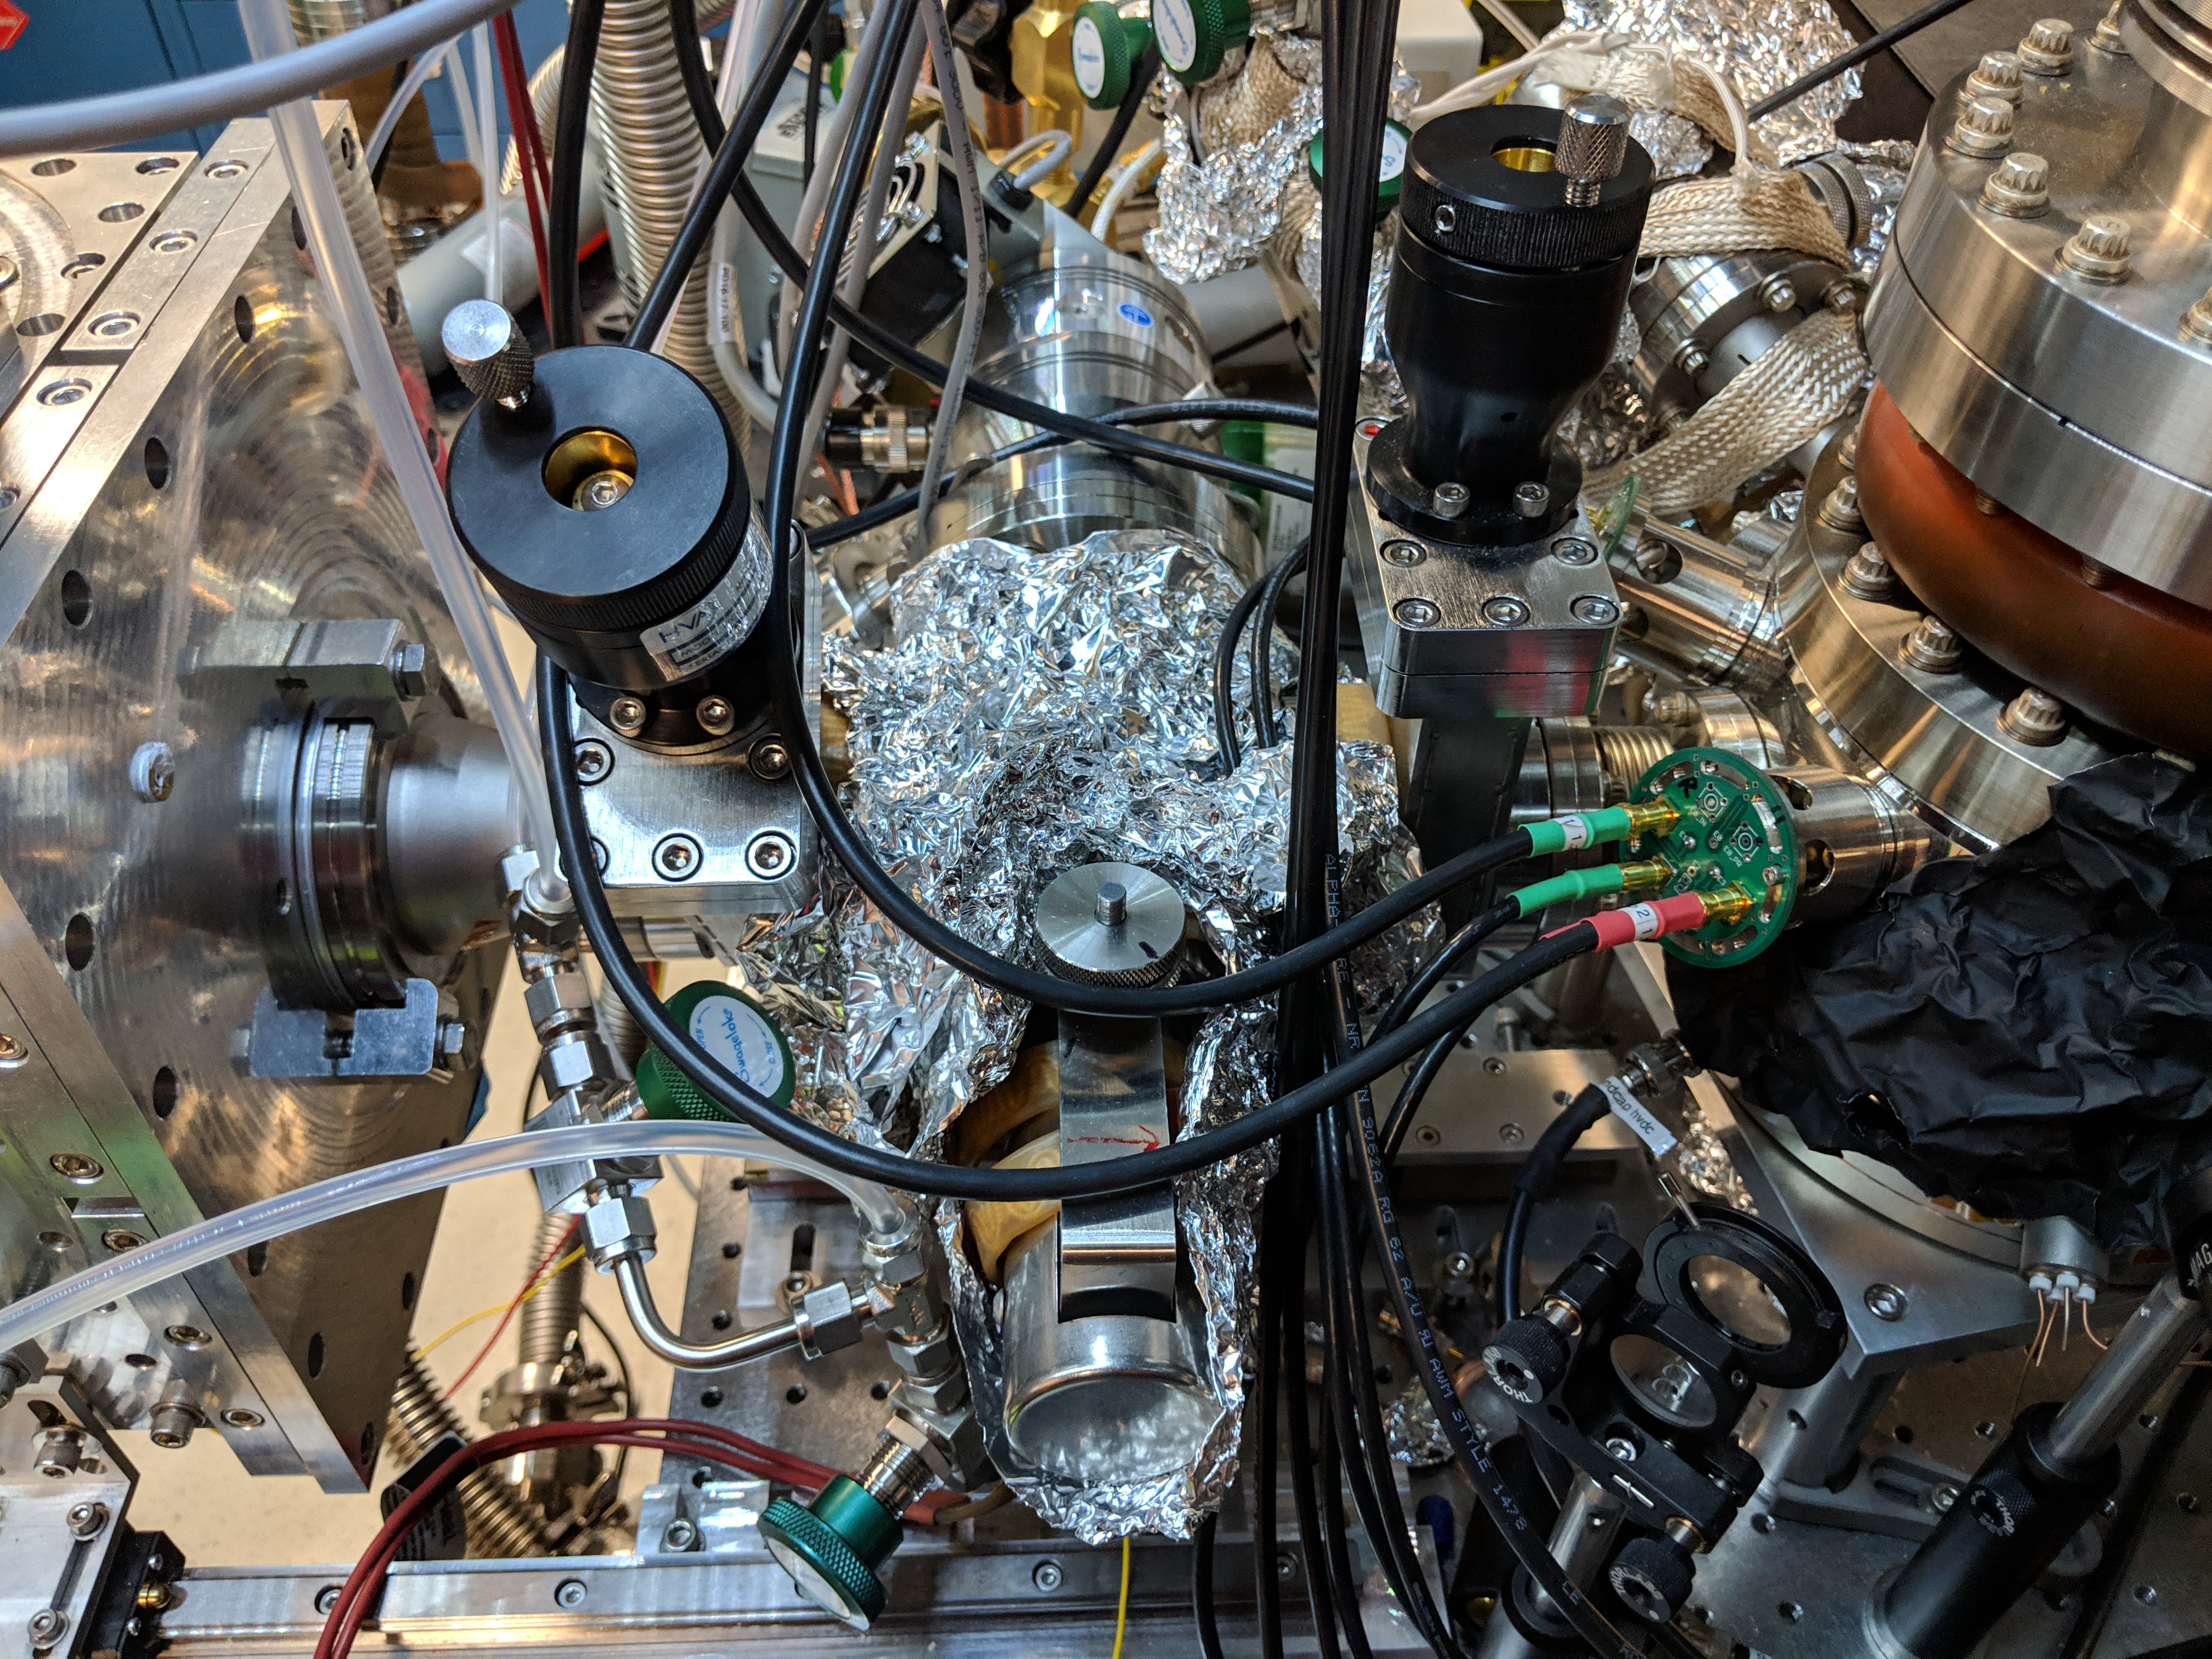
\includegraphics[width=0.8\textwidth]{images/differential_pumping.jpg}
	\caption{Differential pumping region in between the stem and ion trap chambers with gate valves on either end. Blank copper CF gaskets with apertures of 4 mm and 10 mm are placed towards the stem and ion chamber respectively to limit conductance of background gasses while allowing the cryogenic beam through. An Agilent Twistorr 84 FS turbo pump keeps the region at pressures around $10^{-10}$ Torr and a leak valve allows for controlled introduction of secondary gasses.}
	\label{fig: differential pumping}
\end{figure}